\subsection{Infusion}
The redistribution process depends on the ratio of the solubility of the doping material in silicon and SiO$ _2$. At the Si/SiO$ _2$ interface the dopants are redistributed by segregation until the ratio of their concentration at the interface is the same as the ratio of their solubility in both materials. The ratio of dopant solubility is expressed by the segregation coefficient $m$ which is

\begin{equation}
\displaystyle m = \frac{
	\mathrm{solubility\ in\ silicon}
	}{
	\mathrm{solubility\ in\ SiO_2}
	}
\end{equation}

As listed in \autoref{table_diffusion_coeff} below there are dopant species which solubilize better in SiO$ _2$ than in silicon ($ m < 1$) and species which have a reversed behavior ($ m > 1$).
In case of $ m < 1$, as for Boron, the dopant concentration is enhanced at the SiO$ _2$ side, whereas beneath the interface, there is a dopant depletion at the silicon surface.
For reversed solubility ratios ($ m > 1$, like Phosphorus), only few dopant atoms penetrate the interface.
In order to obtain the by $ m$ determined concentration ratio at the interface, dopant atoms from deeper silicon zones diffuse back to the surface zone.
Therefore, the dopant concentration at the silicon surface is enhanced, as illustrated in \autoref{graph_figure}b.
In \autoref{graph_figure} $ C_c$ denotes the dopant concentration in the silicon surface zone before oxidation. $ x$ is the distance from the silicon surface.

\begin{figure}[H]
	\centering
	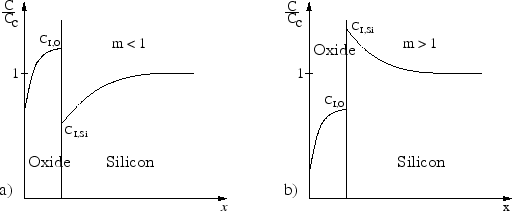
\includegraphics[width=0.75\linewidth]{img349.png}
	\caption{Schematic illustration of dopant redistribution}
	\label{graph_figure}
\end{figure}
\begin{table}[H]
	\centering
	\begin{tabular}{|c|c|c|c|c|c|}
		\hline
		Dopant species &
		Boron &
		Phosphor &
		Antimon &
		Arsen &
		Gallium \\
		\hline
		$m$ &
		0.1-0.3 &
		10 &
		10 &
		10 &
		20 \\
		\hline
	\end{tabular}
	\caption{Segregation coefficients $m$ for important dopant species in silicon}
	\label{table_diffusion_coeff}
\end{table}
